\documentclass[12pt,a4paper]{article}

\usepackage[french]{babel}
\usepackage[utf8]{inputenc}
\usepackage[T1]{fontenc}
\usepackage[a4paper,top=2cm,bottom=2cm,left=3cm,right=3cm]{geometry}
\usepackage{graphicx}
\usepackage{wrapfig}
\usepackage{booktabs}
\usepackage{amsmath}

% liens en bleu
\usepackage[colorlinks=true,
            linkcolor=blue,
            urlcolor=blue,
            citecolor=blue]{hyperref}

\usepackage{float}
\usepackage{titling}
\setlength{\droptitle}{-4em}
\pretitle{\begin{center}\LARGE\bfseries}
\posttitle{\par\vskip 1.5em\end{center}}
\preauthor{\begin{center}\large}
\postauthor{\par\end{center}}
\predate{\begin{center}\large}
\postdate{\par\end{center}}

\usepackage{fancyhdr}
\pagestyle{fancy}
\fancyhf{}
\rhead{\leftmark}
\lhead{Projet CPES2}
\rfoot{\thepage}

\title{Rapport Projet CPES2 2025\\Analyse de données sous R}
\author{%
  \href{https://www.linkedin.com/in/utharushan/}{\textbf{UTHAYAKUMAR Tharushan}}\\[0.5em]
  \href{mailto:tharushan.uthayakumar@hec.edu}{tharushan.uthayakumar@hec.edu}
}
\date{23 mai 2025}

\begin{document}
\begin{titlepage}
  \centering
  \vspace*{2cm}
  {\LARGE\bfseries Rapport Projet CPES2 2025\par}
  \vspace{1em}
  {\Large Analyse de données sous R\par}
  \vfill
  {\large\textbf{UTHAYAKUMAR Tharushan}\par}
  \vspace{0.5em}
  {\small\href{mailto:tharushan.uthayakumar@hec.edu}{tharushan.uthayakumar@hec.edu}\par}
  \vspace{1em}
  {\small\href{https://github.com/Utharushan/Projet-Final-Intro-a-R-CPES-Saclay}{Dépôt GitHub associé}\par}
  \vfill
  {\normalsize 23 mai 2025\par}
\end{titlepage}

\begin{abstract}
Ce rapport présente deux analyses distinctes réalisées sous R (version 4.5.0) :
\begin{itemize}
  \item \textbf{Partie A} : étude de l'influence de la température moyenne sur le pic journalier de consommation électrique (2012--2025), via une régression linéaire simple, révélant une relation négative forte (R\textsuperscript{2} = 0,69).
  \item \textbf{Partie B} : exploration des données d'effectifs de patients par pathologie, sexe, classe d'âge et territoire (départements, régions), avec visualisations (cartes, heatmaps, évolutions temporelles), afin de décrire la répartition et les tendances des prévalences.
\end{itemize}
Les méthodologies font appel aux packages \texttt{ggplot2}, \texttt{dplyr}, \texttt{lubridate}, \texttt{sf} et \texttt{viridis}. Le code est disponible sur le dépôt GitHub ci-dessus.
\end{abstract}

\newpage
\tableofcontents
\newpage

\section*{Introduction}
Le présent document propose deux volets d'analyse de données réalisés en langage R. Chaque partie décrit les données, la préparation, la méthodologie suivie, les résultats obtenus et les principales conclusions.

\section{Partie A -- Pic journalier de la consommation brute d'électricité}
\subsection{Contexte et objectif}
Le premier jeu de données (accessible sur \href{https://www.data.gouv.fr/fr/datasets/pic-journalier-de-la-consommation-brute-delectricite/}{data.gouv.fr}) couvre la période 2012--2025 et fournit pour chaque date :
\begin{itemize}
  \item le pic journalier de consommation électrique en MW,
  \item la température moyenne observée (Temp\_moy, °C),
  \item la température climatologique de référence (Temp\_ref, °C).
\end{itemize}
L'objectif est de quantifier l'impact de la température moyenne sur la consommation à l'aide d'un modèle de régression linéaire simple.

\subsection{Méthodologie}
\subsubsection{Environnement et packages}
Analyse réalisée sous R 4.5.0, avec :
\begin{itemize}
  \item \texttt{ggplot2} pour les visualisations,
  \item \texttt{dplyr} et \texttt{lubridate} pour la préparation et la manipulation,
  \item \texttt{scales} pour le formatage des axes.
\end{itemize}

\subsubsection{Préparation des données}
Lectures, conversion de la colonne \texttt{Date}, calcul de moyennes mensuelles, et vérification des valeurs manquantes.

\subsection{Exploration visuelle}

\begin{figure}[H]
  \centering
  \begin{minipage}[t]{0.9\textwidth}
    \centering
    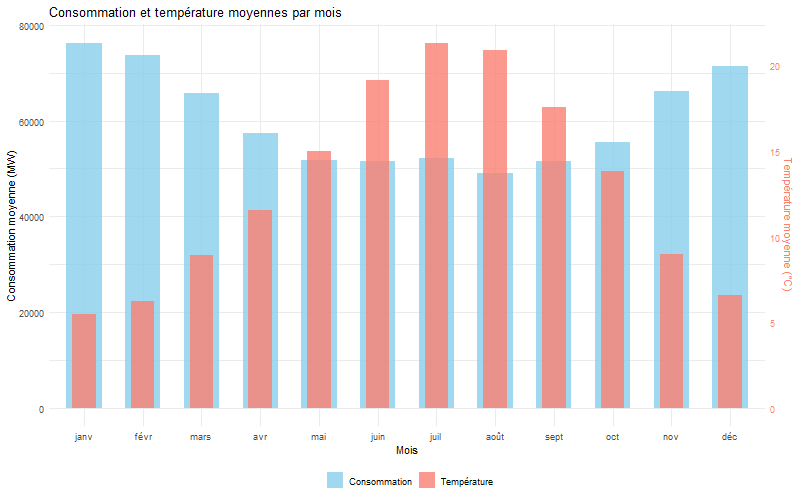
\includegraphics[width=\linewidth]{Projet_partie_A/conso_temp_moyennes_par_mois_superpose.png}
    \caption{Consommation et température moyennes par mois}
    \label{fig:conso_temp_mois}
  \end{minipage}
    \begin{itemize}
      \item Les mois froids (janv.–fév.) ont une basse température et une haute consommation.  
      \item En été (juil.–août), température élevée et consommation minimale.  
      \item Confirme l’impact direct de la température sur la demande électrique.  
    \end{itemize}
\end{figure}

\begin{figure}[H]
  \centering
  \begin{minipage}[t]{0.9\textwidth}
    \centering
    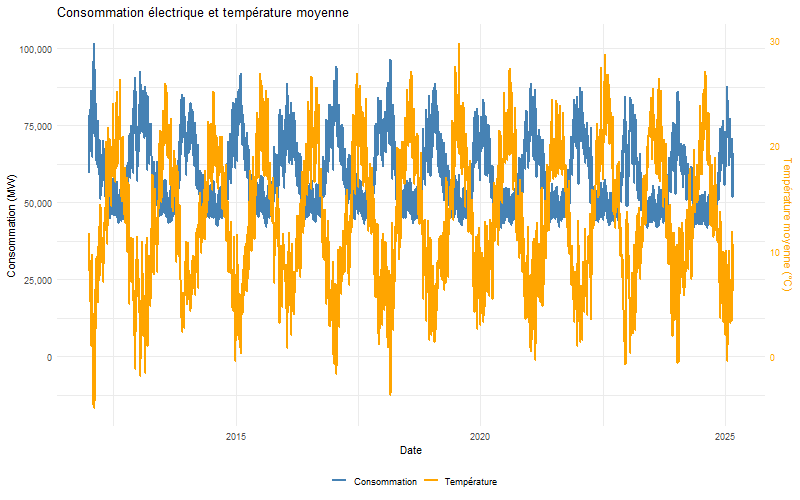
\includegraphics[width=\linewidth]{Projet_partie_A/conso_vs_temp_superpose.png}
    \caption{Superposition Consommation \& Température (2012–2025)}
    \label{fig:timeseries_conso_temp}
  \end{minipage}
    \begin{itemize}
      \item Cycles saisonniers opposés : consommation haute quand température basse et vice-versa.  
      \item Calage immédiat, illustrant une dépendance sans délai notable.  
    \end{itemize}
\end{figure}

\subsection{Modèle de régression linéaire}
Le modèle ajusté sur $n = 3652$ jours se formule ainsi :
\[
\widehat{\text{Conso}}
= \beta_0 + \beta_1\,\times\,\text{Temp\_moy} + \varepsilon.
\]
Les résultats du modèle sont présentés dans le tableau ci‑dessous :

\begin{table}[H]
  \centering
  \begin{tabular}{lrrrr}
    \toprule
                 & \textbf{Estimate} & \textbf{Std. Error} & \textbf{t value} & \textbf{Pr(>|t|)} \\
    \midrule
    (Intercept)  & 79\,642.0         & 209.0               & 381.4            & $<2\times10^{-16}$ \\
    Temp\_moy    & $-1\,496.4$       & 14.5                & $-102.9$         & $<2\times10^{-16}$ \\
    \bottomrule
  \end{tabular}
  \caption{Coefficients du modèle de régression linéaire simple}
  \label{tab:reglin}
\end{table}

\paragraph{Qualité de l’ajustement}
\begin{itemize}
  \item $R^2 = 0.688$, $R^2_{\mathrm{adj}} = 0.688$: la température moyenne explique 68,8\,\% de la variance du pic de consommation.
  \item Statistique $F = 1{,}06 \times 10^4$ (ddl : 1 et 3650), $p-valeur < 2{,}2\times10^{-16}$ : rejet très significatif de l’hypothèse nulle $H_0: \beta_1 = 0$, ce qui confirme l’existence d’une relation linéaire entre température et consommation.
  \item Le coefficient $\beta_1 = -1\,496.4$ indique qu’une augmentation de la température moyenne d’un degré Celsius est associée, en moyenne, à une baisse d’environ $1\,500\,$MW du pic journalier de consommation.
\end{itemize}

\subsection{Conclusions Partie A}
La température moyenne du jour est un prédicteur fort du pic de consommation, expliquant près de 69\,\% de sa variabilité.  
Pour approfondir l’analyse, on pourrait :
\begin{itemize}
  \item Intégrer des variables calendaires (week‑ends, jours fériés).
  \item Ajouter des indicateurs saisonniers ou des paramètres météorologiques complémentaires (humidité, vent).
  \item Passer à une régression multiple pour isoler l’impact de la température des autres facteurs.
\end{itemize}
\newpage
\section{Partie B -- Pathologies : effectifs par territoire, âge et sexe}
\subsection{Contexte et objectif}
Le second jeu de données (accessible sur \href{https://data.ameli.fr/explore/dataset/effectifs/information/}{data.ameli.fr}) présente pour les années 2019--2022 :
\begin{itemize}
  \item les effectifs de patients par pathologie,
  \item par classe d'âge, sexe, département et région,
  \item avec pour chaque groupe la prévalence en pourcentage.
\end{itemize}
L'objectif est d'analyser la distribution et l’évolution temporelle des prévalences pour les principales pathologies,  
en mettant en évidence les disparités selon l’âge, le sexe et le territoire, afin d’orienter d’éventuelles actions de santé publique. 

\subsection{Méthodologie}
\begin{itemize}
  \item Préparation et nettoyage : filtrage des valeurs manquantes, renommage des variables.
  \item Cartographie : shapefile des régions, fusion avec la prévalence et rognage sur la métropole.
  \item Visualisations : barplots, heatmaps, évolutions temporelles, boxplots, scatterplots, pie charts.
\end{itemize}

\subsection{Exploration visuelle}

\begin{figure}[H]
  \centering
  \begin{minipage}[t]{0.6\textwidth}
    \centering
    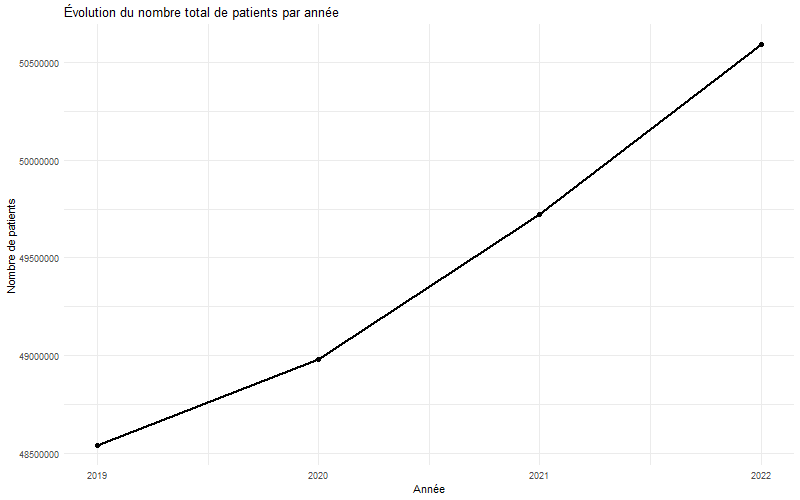
\includegraphics[width=\linewidth]{Projet_partie_B/01_total_patients_par_annee.png}
    \caption{Évolution du nombre total de patients par année}
    \label{fig:total_patients}
  \end{minipage}
    \begin{itemize}
      \item Une augmentation quasi linéaire du total de patients, passant d’environ 48,5 M en 2019 à 50,5 M en 2022.  
      \item Un signal régulier sans plateau, suggérant une croissance continue de la demande de soins ou de la couverture de données.  
      \item L’absence de point d'inflexion indique aucune rupture majeure (crise sanitaire ou changement de méthodologie).  
    \end{itemize}
\end{figure}

\begin{figure}[H]
  \centering
  \begin{minipage}[t]{0.7\textwidth}
    \centering
    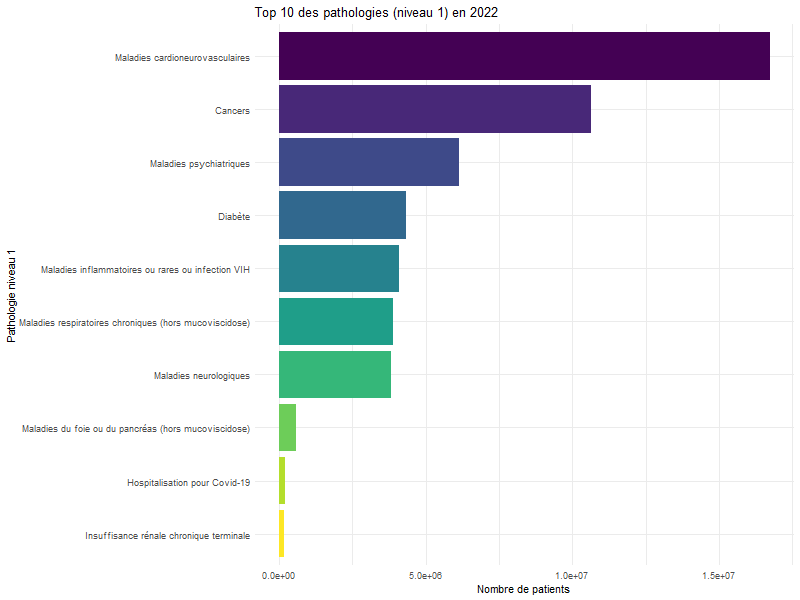
\includegraphics[width=\linewidth]{Projet_partie_B/02_top10_patho1.png}
    \caption{Top 10 des pathologies (niv.1) en 2022}
    \label{fig:top10_patho}
  \end{minipage}
    \begin{itemize}
      \item Les maladies cardiovasculaires en tête (~16 M de patients), puis cancers (~11 M) et psychiatriques (~7 M).  
      \item Diabète et maladies inflammatoires/VIH autour de 4–5 M, position médiane.  
      \item Insuffisance rénale terminale et hospitalisation pour Covid-19 très marginales.  
    \end{itemize}
\end{figure}

\begin{figure}[H]
  \centering
  \begin{minipage}[t]{0.7\textwidth}
    \centering
    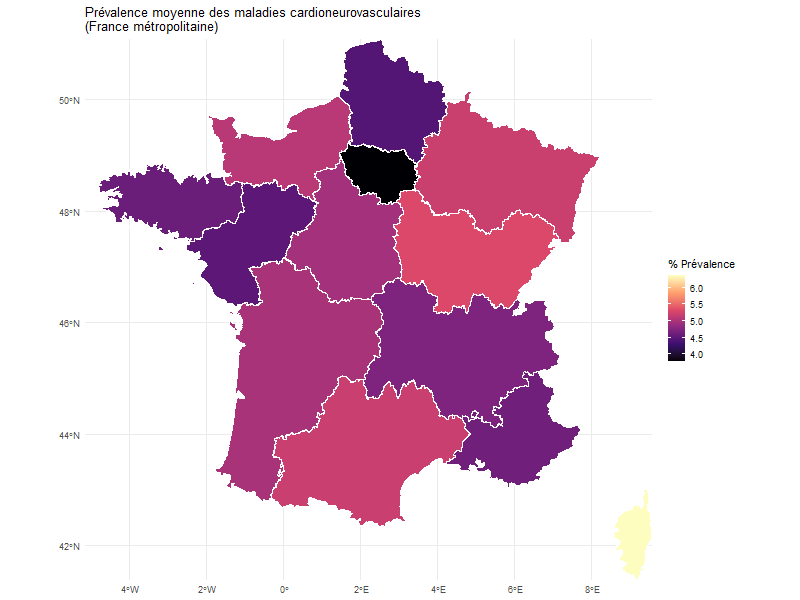
\includegraphics[width=\linewidth]{Projet_partie_B/03_carte_prevalence_par_region_metropolitaine.png}
    \caption{Prévalence des maladies cardiovasculaires (Métropole)}
    \label{fig:carte_prevalence}
  \end{minipage}
    \begin{itemize}
      \item Île-de-France la plus faible (~4 \%), Grand Est et Bourgogne-Franche-Comté élevées (≈5,5 \%).  
      \item Arc Est et Sud-Ouest plus exposés, possiblement dû à des facteurs de risque régionaux.  
      \item Rognage sur la métropole améliore la clarté en supprimant les DOM-TOM.  
    \end{itemize}
\end{figure}

\begin{figure}[H]
  \centering
  \begin{minipage}[t]{1\textwidth}
    \centering
    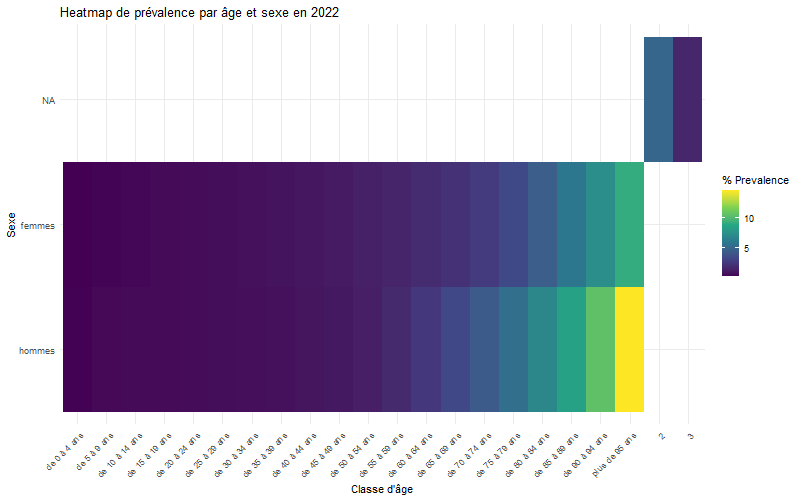
\includegraphics[width=\linewidth]{Projet_partie_B/04_heatmap_age_sexe.png}
    \caption{Heatmap prévalence par âge et sexe en 2022}
    \label{fig:heatmap_age_sexe}
  \end{minipage}
    \begin{itemize}
      \item Croissance exponentielle de la prévalence avec l’âge, de <1 \% (<40 ans) à >10 \% (>85 ans).  
      \item Légère surreprésentation masculine chez les 65 ans et plus.  
      \item Catégorie « tous sexes » (NA) regroupe des valeurs intermédiaires, moins discriminantes.  
    \end{itemize}
\end{figure}

\begin{figure}[H]
  \centering
  \begin{minipage}[t]{0.8\textwidth}
    \centering
    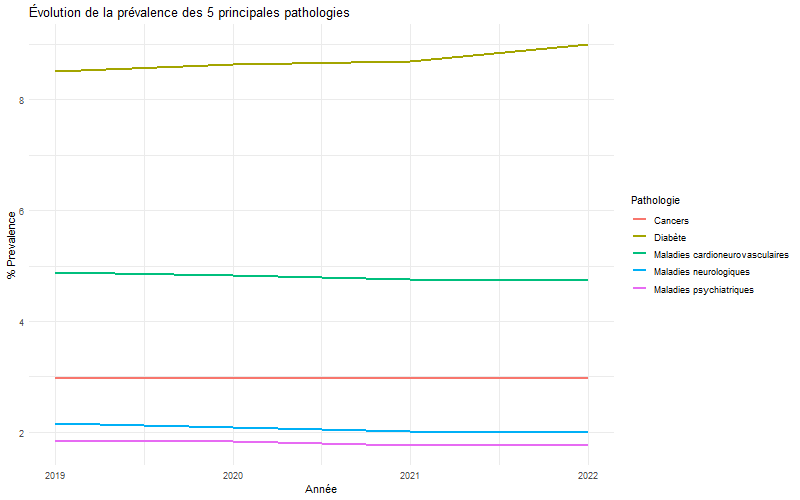
\includegraphics[width=\linewidth]{Projet_partie_B/05_evol_prev_top5.png}
    \caption{Évolution de la prévalence des 5 pathologies principales}
    \label{fig:evol_prev_top5}
  \end{minipage}
  \hfill
    \begin{itemize}
      \item Diabète en hausse (de ~8,5 \% à ~9 \%), indicateur de progression continue.  
      \item Cardioneurovasculaires stables ~5 \%, cancers (~3 \%), neurologiques (~2 \%) et psychiatriques (~1,8 \%) en légère baisse.  
      \item Différentes dynamiques suggèrent des évolutions distinctes d’incidence ou de prise en charge.  
    \end{itemize}
\end{figure}

\begin{figure}[H]
  \centering
  \begin{minipage}[t]{1\textwidth}
    \centering
    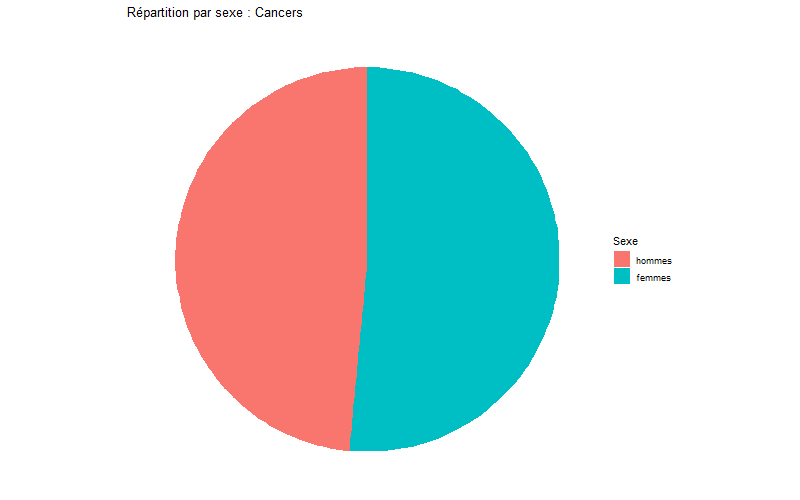
\includegraphics[width=0.6\linewidth]{Projet_partie_B/07_pie_sexe_patho.png}
    \caption{Répartition hommes/femmes pour « Cancers »}
    \label{fig:pie_sexe}
  \end{minipage}
    \begin{itemize}
      \item Légère prédominance féminine (~52 \%) parmi les patients atteints de cancers.  
      \item Répartition presque équilibrée, reflétant la distribution par sexe selon les types de cancer.  
    \end{itemize}
\end{figure}

\begin{figure}[H]
  \centering
  \begin{minipage}[t]{1.2\textwidth}
    \centering
    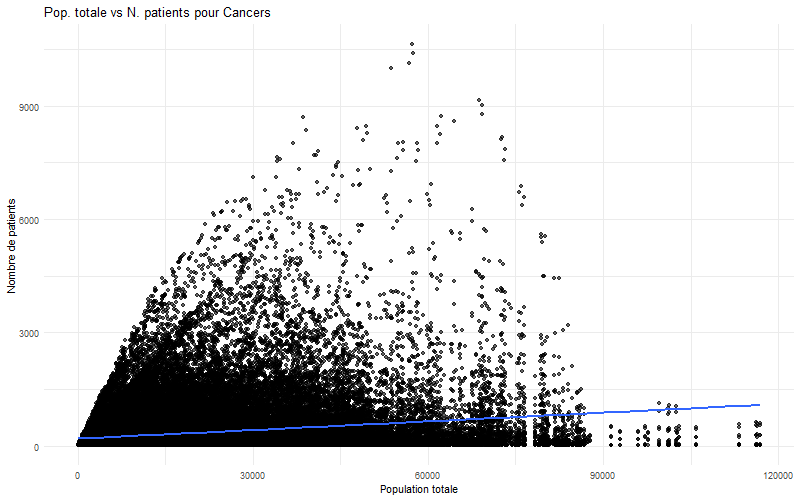
\includegraphics[width=\linewidth]{Projet_partie_B/08_scatter_pop_vs_patients.png}
    \caption{Population vs nombre de patients (Cancers)}
    \label{fig:scatter_pop_patients}
  \end{minipage}
    \begin{itemize}
      \item Corrélation positive mais dispersion forte : plus de population, plus de cas, mais variabilité importante. 
      \item Pente de régression faible : +10 000 hab ≈ +200 cas, dépendance modérée.  
      \item Territoires très peuplés montrent des prévalences hétérogènes.  
    \end{itemize}

\end{figure}

\begin{figure}[H]
  \centering
  \begin{minipage}[t]{0.8\textwidth}
    \centering
    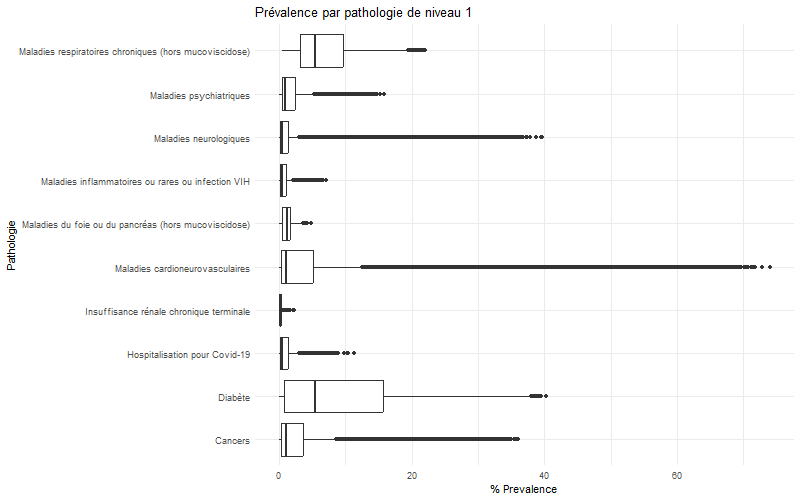
\includegraphics[width=\linewidth]{Projet_partie_B/09_boxplot_patho1.png}
    \caption{Prévalence par pathologie (niv.1)}
    \label{fig:boxplot_patho1}
  \end{minipage}
    \begin{itemize}
      \item Diabète : Ecart Interquartile large (4–20 \%), plus de variabilité départementale.  
      \item Cardioneurovasculaires avec outliers extrêmes (>60 \%).
      \item Insuffisance rénale et Covid-19 très concentrées à faible taux (<5 \%).  
    \end{itemize}
\end{figure}

\subsection{Conclusions Partie B}
\begin{itemize}
  \item Les maladies cardioneurovasculaires et les cancers restent les pathologies les plus fréquentes, avec respectivement plus de 16 M et 11 M de patients en 2022, tandis que le diabète présente une prévalence approchant 9 \%.  
  \item La cartographie révèle des disparités régionales marquées : certaines zones métropolitaines (Grand Est, Bourgogne‑Franche‑Comté, Hauts‑de‑France) enregistrent des prévalences plus élevées que la moyenne nationale.  
  \item La heatmap par âge et sexe montre une progression régulière de la prévalence avec l’âge et une légère prédominance masculine chez les seniors.  
  \item L’évolution temporelle (2019–2022) met en évidence une montée constante du diabète, alors que les autres pathologies se stabilisent ou varient faiblement.  
  \item Les distributions départementales confirment une forte hétérogénéité locale, avec des outliers indiquant des territoires à risque accru.  
\end{itemize}

\section*{Conclusions Globales}
Cette étude illustre la puissance de R pour l’analyse statistique.  
\begin{itemize}
  \item \textbf{Partie A :} la régression simple montre que la température moyenne explique près de 69 \% de la variabilité du pic de consommation électrique, soulignant l’importance du prévisionnel hivernal.  
  \item \textbf{Partie B :} l’exploration des données de santé met en lumière les pathologies prioritaires, leurs disparités géographiques, et leurs évolutions démographiques.  
\end{itemize}
Les approches graphiques (séries temporelles, heatmaps, cartographies) et modélisation fournissent une base solide pour orienter les décisions en politique énergétique et en santé publique.  


\newpage

\section{ANNEXE}

\subsection{Graphiques supplémentaires Partie A}

\begin{figure}[H]
  \centering
  \begin{minipage}[t]{0.48\textwidth}
    \centering
    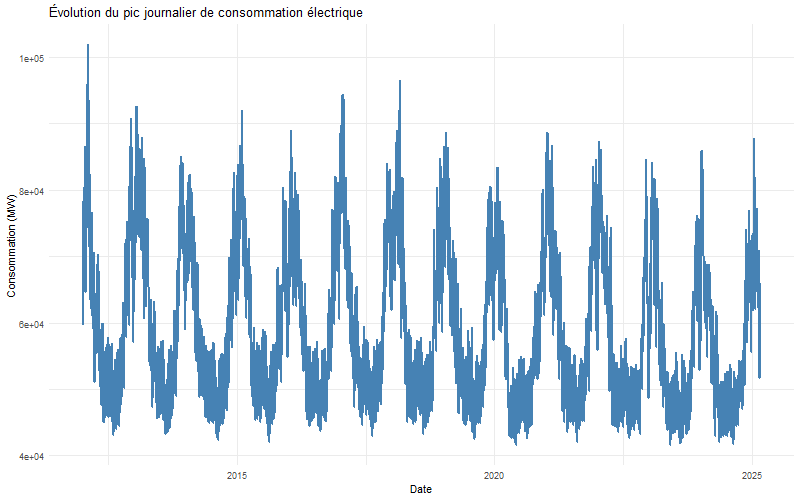
\includegraphics[width=\linewidth]{Projet_partie_A/graphique_conso.png}
    \caption{Pic journalier de consommation électrique (2012–2025)}
    \label{fig:conso_journaliere}
  \end{minipage}
  \hfill
  \begin{minipage}[t]{0.48\textwidth}
    \begin{itemize}
      \item Cycle annuel marqué : pointes >95 000 MW en hiver, creux ≈45 000–50 000 MW en été.  
      \item Légère tendance haussière des maxima hivernaux, suggérant une hausse de la demande de chauffage ou d’équipement.  
    \end{itemize}
  \end{minipage}
\end{figure}

\begin{figure}[H]
  \centering
  \begin{minipage}[t]{0.48\textwidth}
    \centering
    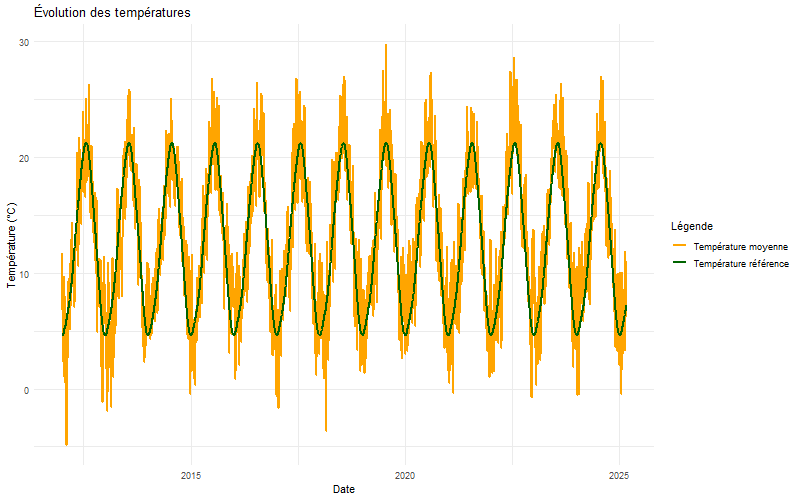
\includegraphics[width=\linewidth]{Projet_partie_A/graphique_temps.png}
    \caption{Température moyenne vs référence (2012–2025)}
    \label{fig:temps_vs_ref}
  \end{minipage}
  \hfill
  \begin{minipage}[t]{0.48\textwidth}
    \small
    \begin{itemize}
      \item Température observée (orange) et de référence (verte) très alignées, avec oscillations journalières/saisonnières.  
      \item Max ≈25–30 °C en été, min parfois <0 °C en hiver ; interannuel stable.  
    \end{itemize}
  \end{minipage}
\end{figure}

\begin{figure}[H]
  \centering
  \begin{minipage}[t]{0.48\textwidth}
    \centering
    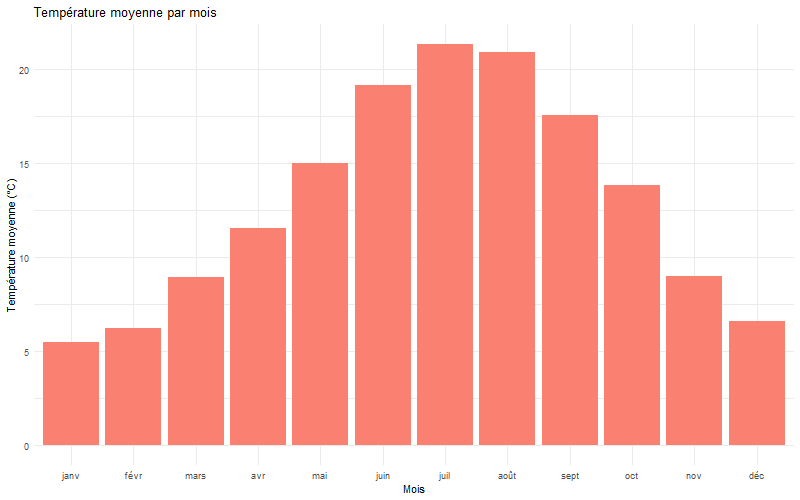
\includegraphics[width=\linewidth]{Projet_partie_A/temp_moyenne_par_mois.png}
    \caption{Température moyenne par mois}
    \label{fig:temp_moyenne_mois}
  \end{minipage}
  \hfill
  \begin{minipage}[t]{0.48\textwidth}
    \small
    \begin{itemize}
      \item Montée linéaire de ~5 °C (janv.) à ~22 °C (juil.), puis redescente symétrique.  
      \item Forte saisonnalité, avec gradient régulier entre saisons.  
    \end{itemize}
  \end{minipage}
\end{figure}

\begin{figure}[H]
  \centering
  \begin{minipage}[t]{0.48\textwidth}
    \centering
    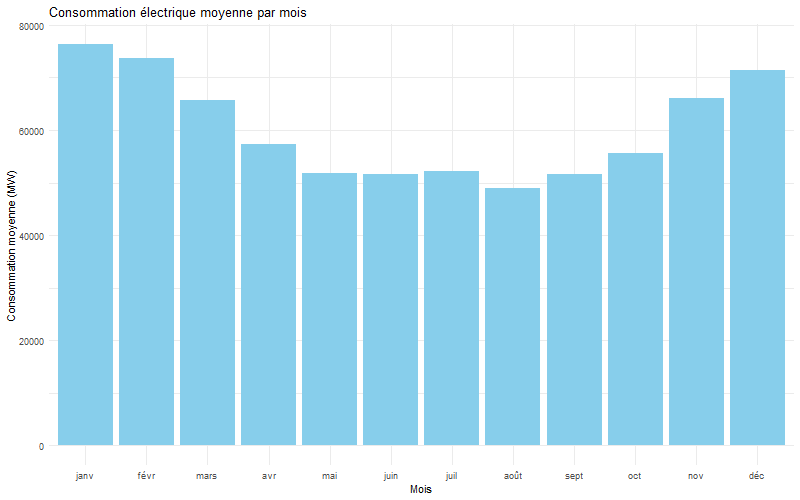
\includegraphics[width=\linewidth]{Projet_partie_A/conso_moyenne_par_mois.png}
    \caption{Consommation moyenne par mois}
    \label{fig:conso_moyenne_mois}
  \end{minipage}
  \hfill
  \begin{minipage}[t]{0.48\textwidth}
    \small
    \begin{itemize}
      \item Profil en « U » : haute consommation en janv.–fév. (~75–78 kMW), creux en août (~49 kMW), puis remontée.  
      \item Corrélation inverse avec la température, traduisant un usage de chauffage en hiver.  
    \end{itemize}
  \end{minipage}
\end{figure}

\begin{figure}[H]
  \centering
  \begin{minipage}[t]{0.48\textwidth}
    \centering
    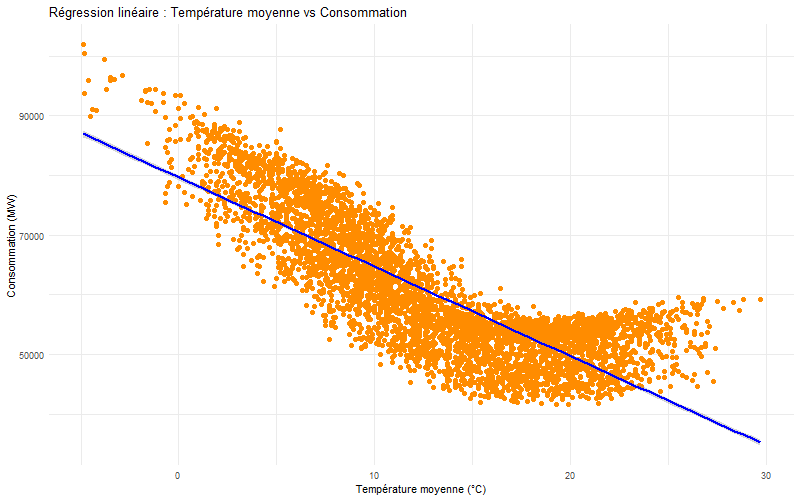
\includegraphics[width=\linewidth]{Projet_partie_A/regression_temp_vs_conso.png}
    \caption{Régression : Température vs consommation}
    \label{fig:regression_temp_conso}
  \end{minipage}
  \hfill
  \begin{minipage}[t]{0.48\textwidth}
    \small
    \begin{itemize}
      \item Relation linéaire négative forte (pente ≈–1 500 MW/°C).  
      \item Dispersion autour de la droite faible, confirmant la fiabilité du modèle.  
      \item 3 652 points journaliers illustrant une robustesse statistique.  
    \end{itemize}
  \end{minipage}
\end{figure}

\subsection{Graphiques supplémentaires Partie B}

\begin{figure}[H]
  \centering
  \begin{minipage}[t]{0.48\textwidth}
    \centering
    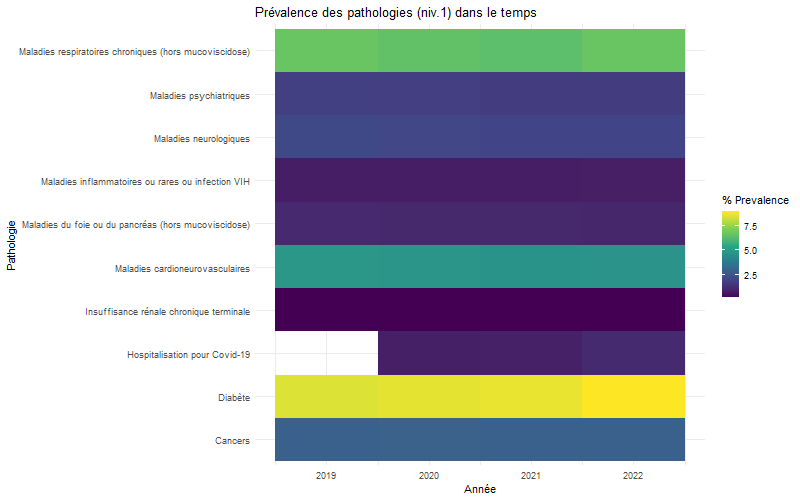
\includegraphics[width=\linewidth]{Projet_partie_B/10_heatmap_patho_temps.png}
    \caption{Heatmap temporelle des prévalences (2019–2022)}
    \label{fig:heatmap_temps}
  \end{minipage}
  \hfill
  \begin{minipage}[t]{0.48\textwidth}
    \small
    \begin{itemize}
      \item Diabète en nette hausse de 2019 à 2022.  
      \item Cancers stables et légèrement croissants, cardiovasculaires constants avec un léger creux en 2021.
    \end{itemize}
  \end{minipage}
\end{figure}

\end{document}
